% !TeX root = RJwrapper.tex

\title{\pkg{BayesSPsurv}: An R Package to Estimate Bayesian (Spatial) Split-Population Survival Models}
\author{by Brandon Bolte, Nicol\'as Schmidt, Sergio B\'ejar, Nguyen Huynh, Bumba Mukherjee}

\maketitle


\abstract{Survival data often include a fraction of units that are susceptible to an event of interest as well as a fraction of “immune” units. In many applications, spatial clustering in unobserved risk factors across nearby units can also affect their survival rates and odds of becoming immune. To address these methodological challenges, this article introduces our \CRANpkg{BayesSPsurv} R-package, which fits parametric Bayesian Spatial split-population survival (cure) models that can account for spatial autocorrelation in both subpopulations of the user’s time-to-event data. Spatial autocorrelation is modeled with spatially weighted frailties, which are estimated using a conditionally autoregressive prior. The user can also fit parametric cure models with or without nonspatial i.i.d. frailties, and each model can incorporate time-varying covariates. \pkg{BayesSPsurv} also includes various functions to conduct pre-estimation spatial autocorrelation tests, visualize results, and assess model performance, all of which are illustrated using data on post-civil war peace survival.}

\section{Introduction}
Conventional survival models have been applied to analyze time-to-event data across several academic disciplines, but these models rely on two core assumptions that are not always tenable. The first is that all units, including right-censored observations, will eventually experience the event of interest. In many applications, however, some fraction of subjects that are “immune” or “cured” may never experience the event \citep{maller1996survival,peng2014cure,beger2017splitting}. A clinical study of obesity on human death rates can employ a standard survival model because all subjects will eventually die, but a study on vaccine effectiveness will likely assume that some fraction of the treated population will become immune while others may respond differently and remain uncured. To account for both subpopulations, scholars have developed a class of split-population (SP) survival models that probabilistically separate the immune fraction from the units that are susceptible to the event of interest and then estimate the conditional hazard of survival among the latter units \citep{smcure-package,spduration-pkg, box1999modeling, boxsteffbook}. The second assumption of conventional survival models is that each observation is conditionally independent after controlling for covariates. This assumption is violated if spatially clustered units share common unobserved features that influence their baseline risk of experiencing an event  \citep{darmofal2009bayesian, taylor2017spatsurv}. If spatial autocorrelation matters for process survival and/or the probability of being immune to an event, ignoring it can lead to biased parameter estimates. 

Although there are numerous methods for dealing with spatially autocorrelated time-to-event data (e.g., \citealp{li2002modeling,banerjee2003frailty, henderson2002modeling, spBayesSurv-article}), these spatial survival models do not differentiate between at-risk and immune observations. Conversely, existing SP survival models either ignore spatial autocorrelation altogether or only account for it in the survival stage \citep{banerjee2004parametric}. We present the \pkg{BayesSPsurv}  \citep{BayesSPsurv} R-package (available at \url{https://CRAN.R-project.org/package=BayesSPsurv}), which has the power to overcome these limitations as well as the flexibility for researchers to model spatial clustering in their survival data however they choose to define it. In particular, \pkg{BayesSPsurv} allows the user to estimate parametric Bayesian Spatial split-population survival (cure) models with spatial frailties in both the model's split and survival stages. These models account for spatial clustering in the immune and at-risk fractions of the data. The package also includes functions and code for pre-estimation spatial autocorrelation diagnostics, visualizing results, simulating multiple Markov chains, and implementing Markov Chain Monte Carlo (MCMC) estimation routines for SP survival models with independent (exchangeable) or no random effects. The user can also include time-varying covariates in either stage. In the next section, we outline previous work on SP and spatial survival models, including existing packages and their limitations. We then formally develop the Pooled, Exchangeable, and Spatial Bayesian SP survival models before describing the various functions available in the \pkg{BayesSPsurv} package. We demonstrate these functions using replication data from a published study on the survival of post-civil war peace.

\section{Background and other R-packages}

Scholars have identified at least two sources of conditional heterogeneity in survival data that hasve been separately addressed. The first occurs when a subset of the units in the data are immune from experiencing a ``failure'' event, which violates the assumption that even right-censored observations experience the event of interest \citep{box1999modeling, boxsteffbook, beger2017splitting}. Cure rate or split-population (SP) survival models account for this immune fraction by first estimating the probability that right-censored units are immune from an event in a ``split-stage'' and then the time until \emph{at-risk} censored and non-censored units experience the event. Recent work has extended these models to include i.i.d. frailties \citep{peng2011mixture}, time-varying covariates \citep{beger2017splitting}, and account for random right-censoring \citep{patilea2020general}. Split-population survival models have been used to study phenomena, ranging from the survival of breast cancer patients \citep{wang2005gene}, criminal recidivism \citep{schmidt1989predicting}, the risk of coups \citep{beger2017splitting}, and parasite-induced mortality in river salmon \citep{ray2014using}. 

Separately, conventional survival models have been extended to account for spatial autocorrelation among nearby units \citep{banerjee2003frailty, taylor2017spatsurv,spBayesSurv-article}.
These models relax the assumption of spatial independence by incorporating spatially weighted frailties into the survival model’s baseline hazard function. This allows for the possibility that adjacent units share unmodeled risk factors that influence their underlying propensities for experiencing a failure event. Apart from recent advances in modeling spatial frailties in different survival frameworks (e.g. \citealp{diva2008parametric, spBayesSurv-article}), spatial survival models have been applied to analyze, for example, geographically referenced data on leukemia survival \citep{henderson2002modeling}, position announcements by U.S. House members \citep{darmofal2009bayesian}, prostate cancer
\citep{spBayesSurv-article}, and fire service response times \citep{taylor2017spatsurv}.
Despite these considerable methodological developments, far less attention has been dedicated to accounting for spatial autocorrelation in SP survival settings. This is surprising because  spatial autocorrelation between units may influence their probability of being immune and the survival rate among the units at risk of experiencing the failure event simultaneously. \citet{banerjee2004parametric} develop Bayesian spatial cure models but focus on modeling spatial autocorrelation in the survival stage using a conditionally autoregressive (CAR) prior. In fact, these authors emphasize that future research must “include covariates and spatial random effects as regressors in the cure rate portion of the model, instead of just the log-relative risk portion” (274).

In line with these trends in the literature, some R packages fit standard and split-population survival models but do not allow for the incorporation of spatial information. The \CRANpkg{survival} package \citep{survival-package} fits parametric and semiparametric Cox survival models via MLE, whereas \CRANpkg{dynsurv} \citep{dynsurv} fits the Cox Proportional Hazards (PH) model with dynamic coefficients using MCMC methods. Conventional semi-parametric cure models can be estimated via MLE with the \CRANpkg{smcure} \citep{smcure-package} or \CRANpkg{nltm} \citep{nltm} package. The \CRANpkg{flexsurvcure} \citep{flexsurvcure} package fits parametric mixture and non-mixture cure models for time-to-event data, and the \CRANpkg{spduration} package fits parametric SP survival models with time-varying covariates \citep{spduration-pkg}.

A small handful of packages allow the user to incorporate spatial information into their survival models, but \textit{never} in split-population settings. The \CRANpkg{BayesX} package \citep{BayesX} and its associated interface to R \CRANpkg{R2BayesX}  \citep{R2BayesX-pkg} fit spatial survival models and structured additive regression models with spatial frailties.  The \CRANpkg{spBayesSurv} package \citep{spBayesSurv-pkg} fits several Bayesian survival models with spatial frailties that can be formulated on a PH, proportional odds, or AFT scale, all of which can include time-varying covariates. The \CRANpkg{spatsurv} package also fits Bayesian spatial survival models, including a PH model that permits users to incorporate Gaussian process frailties \citep{spatsurv-pkg}. Beyond R, WinBUGS and GeoBUGs code has been developed to fit, for instance, survival and non-mixture cure models with spatial frailties \citep{banerjee2003frailty,banerjee2004spatial,thomas2004geobugs}.  

To our knowledge, our \CRANpkg{BayesSPsurv} package is the first to allow users to fit parametric split-population survival models with not just time-varying covariates but also spatial frailties in both stages. The frailties in the parametric Bayesian spatial SP model are estimated using the CAR prior approach \citep{besag1991bayesian,bernardinelli1995bayesian,banerjee2003frailty,banerjee2004parametric}. \pkg{BayesSPsurv} also includes functions and routines coded in C++ to fit nonspatial parametric SP survival models with exchangeable frailties in the model’s split and survival-stage equation and without any frailties. Statistical inference of the models in \pkg{BayesSPsurv} is conducted via combined MCMC techniques that require little input from users. Our package and supplemental code also provide functions to implement spatial autocorrelation tests, produce country-level adjacency matrices, generate and compare multiple Markov chains, assess convergence, and conduct model comparison. Before outlining the functionality of the package in greater detail, we turn to briefly develop each of the three included Bayesian split-population survival models.


\section{The Bayesian (\emph{Spatial}) split-population survival model}

\subsection{Model development}

Define $i=\{1,2,...N\}$ for the units that may fail or experience an event of
interest in a continuous-time survival dataset. Let $f(t)$ and $F(t)$
represent the probability density function and cumulative distribution
function. The survival distribution is
$S(t)=1-F(t)$, and the hazard rate is $h(t)=\frac{f(t)}{S(t)}$. Some units will
fail during the time period under observation $(\widetilde{C}_{i}=1)$, while
others do not and are \textquotedblleft censored\textquotedblright%
\ $(\widetilde{C}_{i}=0)$. The general likelihood of the conventional
survival model in which all units eventually experience the
event of interest is

\begin{equation}
{\textstyle\prod\limits_{i=1}^{N}}
\left[f\left(t_{i}\right)\right]^{\widetilde{C}_{i}}\left[S\left(t\right)\right]^{1-\widetilde{C}_{i}}.%
\end{equation}


\noindent Suppose that the survival data includes two
subpopulations: an ``at-risk '' fraction that
can fail and an ``immune'' fraction that will
\emph{not} experience the (failure) event of interest \citep{maller1996survival,yin2005cure,beger2017splitting}. When presented with this
data generation process, researchers typically employ split-population
survival (cure) models with or without unit-specific frailties to
simultaneously estimate the probability of observations being in the immune
fraction and the effect of covariates on the hazard of survival among
the at-risk fraction \citep{maller1996survival,lu2010,peng2014cure}.


To understand these models in more detail, consider the split-population
survival model for the duration $t$ that splits the sample into an at-risk and
an immune fraction. Let $\alpha_{i}=Pr(Y_{i}=1)$ be the probability with which
units enter the immune fraction. $\alpha_{i}$ can be estimated via a binary
response function and is defined for the logit case as:

\begin{equation}
\alpha_{i}=\frac{\exp\left(\mathbf{Z}_{i}\boldsymbol{\gamma}+V_{i}\right)}{1+\exp
\left(\mathbf{Z}_{i}\boldsymbol{\gamma}+V_{i}\right)},
\end{equation}


\noindent where $\mathbf{Z}_{i}$ are p2-dimensional covariates, $\boldsymbol{\gamma
}$ \ the parameter vector in $\mathbb{R}^{p_{2}}$, and
$V_{i}\sim N(0,\sigma^{2})$ are the nonspatial i.i.d unit-specific frailties
(random effects). Equation 2 is the split-population model's split-stage
equation, where the unit-specific frailties $V_{i}$, which are
each independent of other individual random effects, account for
unobserved heterogeneity that influences probability $\alpha_{i}$. Let $W_{i}\sim
N(0,\sigma^{2})$ denote the nonspatial i.i.d unit-specific frailties that
capture the possibility that some units are at different risks of experiencing
the event of interest due to unobserved factors. The proportional hazards function of
the SP survival model with nonspatial, unit-specific frailties is


\begin{equation}
h\left(t_{i}|\mathbf{X}_{i}\boldsymbol{\beta},W_{i}\right)=h_{0}\left(t_{i}\right)\omega_{i}%
\exp\left(\mathbf{X}_{i}\boldsymbol{\beta}\right)=h_{0}\left(t_{i}\right)\exp\left(\mathbf{X}%
_{i}\boldsymbol{\beta}+W_{i}\right),
\end{equation}


\noindent where $h_{0}(t_{i})$ is the baseline hazard (e.g., Weibull, log-logistic), $\log\omega_{i}=W_{i}$, $\mathbf{X}_{i}$ is the
p1-dimensional covariates, and $\boldsymbol{\beta}$ the
parameter vector in $\mathbb{R}^{p_{1}}$. We focus on incorporating unit-specific  frailty terms generally because they are most commonly used in the social sciences. However, our approach could plausibly be extended to a shared frailty framework if the researcher believes that the frailties occur in clusters such that within-cluster frailties are correlated while frailties between clusters are independent.


Suppose, however, that the survival data with the two aforementioned subpopulations
should be fit with time-varying covariates. We can re-define this data
with unique ``entry time'' duration as $t0$ and
``exit time'' as duration $t$ for each period at which an
observation is observed. Let $t0_{ij}$ denote unit $i$'s elapsed time since
inception until the beginning of time period $j$, $t_{ij}$ the elapsed time
since that unit's inception until the end of period $j$, and $\tilde{C}%
_{ij}=1$ if that unit fails or is censored ($\tilde{C}_{ij}=0$) at $t_{ij}$.
The probability of survival up until period $j$ is now $S(t0)=1-F(t0)$ where
$F\left(t0\right)=\int_{0}^{t0}f\left(t0\right)$. In this case, both subpopulations contribute to
the log-likelihood of the split-population survival model with nonspatial
i.i.d frailties as:

\begin{equation}
\resizebox{0.94\hsize}{!}{$
\ln L=\sum_{i=1}^{N}\left\{  \widetilde{C}_{ij}\ln \left[
\left(1-\alpha_{ij}\right)\frac{f\left(t_{ij}|\mathbf{X}_{ij}\boldsymbol{\beta},W_{i}%
\right)}{S\left(t0_{ij}|\mathbf{X}_{ij}\boldsymbol{\beta},W_{i}\right)}\right]
+\left(1-\widetilde{C}_{ij}\right)\ln \left[  \alpha_{i}+\left(1-\alpha_{i}%
\right)\frac{S\left(t_{ij}|\mathbf{X}_{ij}\boldsymbol{\beta},W_{i}\right)}{S\left(t0_{ij}%
|\mathbf{X}_{ij}\boldsymbol{\beta},W_{i}\right)}\right]  \right\}$
},
\end{equation}


\noindent where the ``split-stage'' equation is
$\alpha_{ij}=\frac{\exp\left(\mathbf{Z}_{ij}\boldsymbol{\gamma}\text{ }+V_{i}%
\right)}{1+\exp\left(\mathbf{Z}_{ij}\boldsymbol{\gamma}\text{ }\boldsymbol{+}V_{i}\right)}$. $V_{i}$ and $W_{i}$ are the nonspatial frailties. The model's survival
stage estimates the probability of survival prior to the event of interest
conditional upon being at-risk for that event given covariates $\mathbf{X}%
_{ij}$ and the baseline hazard function. If $V_{i}=W_{i}=0$, then (4)
defines the log-likelihood of the "Pooled" SP
survival model (\emph{without} unit-specific frailties) with time-varying
covariates \citep{ibrahim2001bayesian,lu2010}. However, if unobserved unit-specific heterogeneity influences the probability of immunity or survival time, it can be accounted for with
the split and survival-stage frailty terms ($V_{i}$ and $W_{i}$). In a
Bayesian split-population survival framework, these frailties are incorporated into each
stage of the model using the exchangeable normal prior,

\begin{equation}
W_{i}\sim N\left(0,1/\tau\right)\text{ and }V_{i}\sim N\left(0,1/\tau\right)\text{ },%
\end{equation}


\noindent with $\tau$ as the precision parameter
\citep{banerjee2003frailty, banerjee2004parametric}. The prior in (5) is induced by treating each specified unit as exchangeable
rather than assigning weights corresponding to each unit's spatial
relationship to one another \citep{bernardinelli1992,darmofal2009bayesian}.
This Exchangeable split-population survival model is appropriate if each
unit's frailty is presumed to be independent of other individual random
effects. Geographically, for instance, this means that the influence of each
unit-specific frailty on that unit's probability of being immune or its risk
propensity is completely unrelated to the neighboring units' frailties
unobserved effects.

Suppose, however, that independence among the frailties
\emph{cannot} be assumed---that is, that the frailties exhibit spatial
autocorrelation or clustering that influences each units'
propensity for being immune to an event of interest and their survival time if
they are not immune. In a Bayesian split-population survival model, the assumption of
spatial independence is relaxed by assigning spatial weights to the
unit-specific frailties in the model's split and survival stage and then
statistically incorporating these spatially weighted frailties via the
conditionally autoregressive (CAR) prior approach \citep{besag1991bayesian,banerjee2003frailty}. The CAR prior accounts for spatially autocorrelated frailties by allowing the
frailties to be spatially autocorrelated across geographically adjacent units.

To understand how the CAR prior is applied, first note that spatial data often
take the form of a lattice in which a continuous spatial surface is divided
into a grid of units such as counties, districts, or countries. The spatially
weighted frailties are constructed by defining the relevant spatial
relationship among adjacent units (this could, for example, be geographic distance or
contiguity) in an adjacency matrix $\mathbf{A}$
with elements $a_{ii^{\prime}}$. Each element $a_{ii^{\prime}}$ in
$\mathbf{A}$ is given a weight of 1 if units $i$ and $i^{\prime}$ are
``neighbors,'' and 0 if they are not. Once these spatial weights are defined via the matrix $\mathbf{A}$, this
information is then incorporated into the CAR prior, which permits us to model
spatially dependent frailties between these contiguous units. To employ the
CAR\ prior approach in a Bayesian SP survival framework, the
frailties $V_{i}$ are collected into the vector $\mathbf{V=\{}V_{1}%
,....,V_{N}\}$, and $W_{i}$ into $\mathbf{W=\{}W_{1}$\textit{,....,}$W_{N}\}$.
Separate CAR priors are then employed for $\mathbf{V}$ and $\mathbf{W}$, which
implies the following model structure:%

\begin{equation}
\mathbf{V|}\lambda\sim\text{CAR}\left(\lambda\right)\text{ and }\mathbf{W|}\lambda
\sim\text{CAR}\left(\lambda\right).
\end{equation}


\noindent $\lambda$ is the precision parameter
\citep{besag1991bayesian,banerjee2004parametric}. The
CAR$(\lambda)$ prior for $\mathbf{V}$ and $\mathbf{W}$ has a
joint distribution in each case that has been formally characterized by scholars \cite[126]{banerjee2003frailty}.


The resulting conditional distributions of the spatial frailties for $\mathbf{V}$ and
$\mathbf{W}$ are

\begin{equation}
V_{i}|V_{i^{\prime}\neq i}\text{ }\sim\text{ }N\left(\overline{V_{i}},1/\left(\lambda
m_{i}\right)\right),\text{ \ \ }W_{i}|W_{i^{\prime}\neq i}\text{ }\sim\text{ }
N\left(\overline{W_{i}},1/\left(\lambda m_{i}\right)\right).
\end{equation}


\noindent $\overline{W_{i}}=m_{i}^{-1}\sum_{i^{\prime}\text{ }adj\text{ }%
i}W_{i^{\prime}}$ and $\overline{V_{i}}=m_{i}^{-1}\sum_{i^{\prime}\text{
}adj\text{ }i}V_{i^{\prime}}$. $\overline{W}_{i}$ and $\overline{V_{i}}$ are
the averages of the neighboring\ $W_{i^{^{\prime}}\neq i}$ and $V_{i^{^{\prime
}}\neq i}$, respectively, where $i^{\prime}$ $adj$ $i$ denotes that $i^{\prime}$
is adjacent to $i$ given $\mathbf{A}$, and $m_{i}$ is the number of
these adjacencies (\citealp[989]{bernardinelli1992}; \citealp{thomas2004geobugs, banerjee2003frailty}). Incorporating the spatial information in $\mathbf{A}$ in this way accounts for
the possibility that spatially proximate units share common unmodeled factors
that influence their probability of being immune or their
survival time before experiencing the event of interest. Using this CAR prior
approach to address spatial autocorrelation, the Spatial split-population
survival model's log-likelihood is defined by 
substituting $\mathbf{V=}\left\{  V_{i}\right\}$ and $\mathbf{W=}\left\{
W_{i}\right\}  $\ \ in equation 4 (where $\alpha_{ij}=\frac{\exp
\left(\mathbf{Z}_{ij}\boldsymbol{\gamma}\text{ },\mathbf{V}\right)}{1+\exp\left(\mathbf{Z}%
_{ij}\boldsymbol{\gamma}\text{ }\boldsymbol{,}\mathbf{V}\right)}$ is the split-stage equation).


The log-likelihood of the Pooled (non-frailty), Exchangeable (nonspatial
frailty), and Spatial\ split-population (SP) survival models are compatible with any
survival distribution. The \pkg{BayesSPsurv} package, however,
supports MCMC estimation of these models for the Weibull and
log-logistic distributions. Our empirical application below focuses on the Weibull survival distribution. The density, survival, and hazard rate in the Weibull case are%
\begin{equation}
\begin{gathered}
f\left(t_{ij}|\rho,\theta\right)=\rho\theta\left(\theta t_{ij}\right)^{\rho-1}\exp\left(-\left(\theta
t_{ij}\right)^{\rho}\right)\\
S\left(t_{ij}|\rho,\theta\right)=\exp\left(-\left(\theta t_{ij}\right)^{\rho}\right)\text{ and }h\left(t_{ij}
|\rho,\theta\right)=\rho\theta\left(\theta t_{ij}\right)^{\rho-1},
\end{gathered}
\end{equation}
where $\theta=\exp\left(\mathbf{X}_{ij}\boldsymbol{\beta},\mathbf{W}\right)$ for the
Spatial, $\theta=\exp\left(\mathbf{X}_{ij}\boldsymbol{\beta}+W_{i}\right)$ for the
Exchangeable, and $\theta=\exp\left(\mathbf{X}_{ij}\boldsymbol{\beta}\right)$ for the
Pooled split-population Weibull model. The density, survival function and the
hazard rate for the log-logistic case is defined in \citet{Bolte2021}.

\subsection{Bayesian inference}

Following standard practice for Bayesian inference \citep{carlin2000}, we assign the multivariate normal (MVN) prior to $\boldsymbol{\beta
}=\{\beta_{1},...,\beta_{p_{1}}\}$ and $\boldsymbol{\gamma}=\{\gamma
_{1},...,\gamma_{p_{2}}\}$, and the Gamma prior for $\rho$ with shape and
scale parameters $a_{\rho}$ and $b_{\rho}$ for \emph{each} of the three Bayesian
split-population survival models in the \pkg{BayesSPsurv} package.
\begin{equation}
\begin{split} 
\rho\text{ } &  \sim\text{Gamma}\left(a_{\rho},b_{\rho}\right),\text{ \ \ \ }%
\boldsymbol{\beta}\sim\mbox{MVN}_{p_{1}}\left(\mu_{\beta},\Sigma_{\beta}\right),\text{
\ \ \ }\boldsymbol{\gamma}\sim\mbox{MVN}_{p_{2}} \left(\mu_{\gamma},\Sigma_{\gamma
}\right)\\
&  \text{ \ \ \ \ \ \ \ \ \ \ \ \ \ \ \ \ \ \ }\Sigma
_{\beta\text{ }}\sim\text{IW}\left(S_{\beta},\nu_{\beta}\right)\text{;\ \ }\Sigma
_{\gamma\text{ }}\sim\text{IW}\left(S_{\gamma},\nu_{\gamma}\right),
\end{split}
\end{equation}


\noindent where $a_{\rho}$, $b_{\rho}$, $S_{\beta}$, $\nu_{\beta},\ S_{\gamma
}$, $\nu_{\gamma}$ are the hyperparameters. We use Bayesian
hierarchical modeling to estimate $\Sigma_{\beta}$ and $\Sigma_{\gamma}$
employing the Inverse-Wishart ($\mbox{IW}$) distribution when using the MVN (a
weakly informative) prior. For Bayesian MCMC estimation of the
Spatial\ SP\ survival (Weibull) model, we assign the hyperprior $p(\lambda)$ to
$\lambda$ given the CAR prior approach. Specifically, we assign
the Gamma hyperprior $\lambda\sim\mbox{Gamma}(a_{\lambda},b_{\lambda})$ for
$\lambda$ \citep{banerjee2004parametric,darmofal2009bayesian}.\footnote{We specify the vague prior
$\left(a_{\lambda},b_{\lambda}\right)=\left(0.001,1/0.001\right)=\left(0.001,1000\right)$ as done for $\rho$.}
To estimate the Exchangeable SP Weibull model, we assign the (multivariate) normal prior for
the model's split and survival-stage frailties $\left(V_{i},W_{i}\right)$, and the priors defined in (9) for $\boldsymbol{\beta}$, $\boldsymbol{\gamma}$,and $\rho$. To identify the Exchangeable and Spatial SP models'
intercepts, we impose the constraint that the frailties sum to zero ($\sum_{i}V_{i}=0$ and $\sum_{i}W_{i}=0$).

The joint posterior distribution of the Bayesian Spatial
SP survival model with time-varying covariates---our
main model of interest---is
\begin{equation}
\resizebox{0.93\hsize}{!}{$
\begin{aligned}
\pi\left(\boldsymbol{\beta},\boldsymbol{\gamma},\rho,\mathbf{W},\mathbf{V}
,\lambda,\Sigma_{\beta},\Sigma_{\gamma}|  \mathbf{C},\mathbf{X}
,\mathbf{Z},\mathbf{t},\mathbf{t0},\boldsymbol{\gamma}\right)& \quad\mathit{\propto
}\quad L \left(\boldsymbol{\beta},\boldsymbol{\gamma},\rho,\mathbf{W},\mathbf{V}
|\mathbf{C},\mathbf{X},\mathbf{Z},\mathbf{t,t0}\right)\\
 \pi\left(\mathbf{W}|\lambda\right)\pi\left(\mathbf{V}|\lambda\right)&\pi\left({\beta}|\mu_{\beta
},\Sigma_{\beta}\right)\pi\left({\gamma}|\mu_{\gamma},\Sigma_{\gamma}\right)\pi\left(\rho
\right)\pi\left(\lambda\right)\pi\left(\Sigma_{\beta}\right)\pi\left(\Sigma_{\gamma}\right),
\end{aligned}$}
\end{equation}

\noindent where $L\left(\boldsymbol{\beta},\boldsymbol{\gamma}%
,\rho,\mathbf{W},\mathbf{V}|\mathbf{C},\mathbf{X},\mathbf{Z},\mathbf{t,t0}\right)$
is defined in (4) with $\mathbf{V=\{}%
V_{1},....,V_{N}\}$ and $\mathbf{W=\{}W_{1}$\textit{,....,}%
$W_{N}\}$. The density, survival function, and hazard rate for this likelihood
is given by the Weibull (or log-logistic) distribution in our R-package. $\pi\left(\mathbf{W}|\lambda\right)$ and $\pi\left(\mathbf{V}%
|\lambda\right)$ are defined via their respective conditional distributions in (7).
$\pi\left({\beta}|\mu_{\beta},\Sigma_{\beta}\right)$, $\pi\left({\gamma}|\mu_{\gamma}%
,\Sigma_{\gamma}\right)$, and $\pi\left(\rho\right)$ are from (9), $\pi\left(\Sigma_{\beta}\right)$ and $\pi\left(\Sigma_{\gamma}\right)$
are from (10). $\pi\left(\lambda\right)$ is the Gamma hyperprior for the Spatial SP survival model. From (10), we can define the
joint posterior distribution of the time-varying (i) Exchangeable SP survival
model by incorporating the frailties $V_{i}$ and $W_{i}$ (instead of
$\mathbf{W}$, $\mathbf{V}$, and their CAR priors) given by (5) and
(ii) Pooled SP survival model by excluding frailty terms.


The three split-population survival models in \pkg{BayesSPsurv} are each
estimated with an MCMC algorithm for Bayesian inference. Because closed-forms
for the posterior distributions of $\boldsymbol{\beta,\gamma}$ and $\rho$ are
not available, these parameters in each model are updated in the MCMC algorithm
via slice-sampling (with stepout and shrinkage) from their respective full
conditional distribution. The closed form
of the full conditional distributions (e.g., $\pi\left(\Sigma_{\beta}|{\beta}\right)$ and
$\pi\left(\Sigma_{\gamma}|{\gamma}\right)$) and details about slice-sampling
is provided in \citet{Bolte2021}.\footnote{For more information on slice-sampling, see \citet{neal2003slice}.} Further, because the closed-forms for the posterior distributions of
$\lambda,\mathbf{W}$, and $\mathbf{V}$ are not available for the Spatial split-population
survival model, our MCMC algorithm incorporates Gibbs Sampling for
estimating $\lambda$. Our MCMC update scheme then employs the Metropolis-Hastings algorithm for estimating $\mathbf{V}$ given $\lambda$ and then uses the Metropolis-Hastings algorithm to estimate $\mathbf{W}$ given $\lambda$.\footnote{The closed-form of the
full conditional distribution of $\pi(\lambda|\mathbf{W},\mathbf{V})$ used for
the MCMC update scheme is formally characterized in \citet{Bolte2021}.} In the Exchangeable SP
survival model, the nonspatial i.i.d frailties $V_{i}$ and $W_{i}$  are
updated via Metropolis-Hastings, while the Pooled SP model excludes
frailty terms. The MCMC update scheme to fit each model in \pkg{BayesSPsurv} are
described in detail in \citet{Bolte2021}.



\section{Using the \pkg{BayesSPsurv} R package}

Each of the three Bayesian SP survival models in \pkg{BayesSPsurv} incorporates a cure rate fraction and assumes that the time-to-event baseline hazard follows a Weibull or log-logistic distribution (which the user specifies). Users can also incorporate time-varying covariates in either stage. \pkg{BayesSPsurv} contains compiled C++ code using the package \CRANpkg{Rcpp} \citep{Rcpp-pkg} to maximize computational efficiency when estimating the included Bayesian SP survival models. In addition to the pre-estimation spatial autocorrelation (Join Count and
Global Moran's I) tests described below, the \pkg{BayesSPsurv} package also permits users to calculate the deviance information criterion (DIC) and log-likelihood statistics from the Spatial, Exchangeable, and Pooled SP survival models' MCMC output. The DIC is a measure of model fit that also penalizes the effective number of parameters. Like the Akaike Information Criterion, models with smaller values are preferable to those with larger values. Users can also conduct MCMC diagnostics with various extant packages designed to handle \code{mcmc} objects such as \CRANpkg{coda} \citep{coda-manual}.



\begin{table}[!htb] \centering
\fontsize{9}{12}\selectfont

\begin{tabular}{ll} 
\toprule
Function & Description \\ \midrule 
\code{spatialSPsurv()}  & Fits Bayesian Spatial SP survival model\\
\code{exchangeSPsurv()} & Fits Bayesian Exchangeable SP survival model\\
\code{pooledSPsurv()}   & Fits Bayesian Pooled SP survival model\\
\code{plot\_JoinCount()} & Implement and plot Join Count statistics\\
\code{plot\_Moran.I()} & Implement and plot global Moran's I statistics\\
\code{spatial\_SA()} & Generate spatial weights (adjacency) matrix\\
\code{SPstats()} & Calculate DIC and log-likelihood from fitted models \\ \bottomrule
\end{tabular}
\caption{Functions in the \pkg{BayesSPsurv} package.}
\label{table1}
\end{table}



\subsection{Loading the package, dataset, and assessing spatial autocorrelation}

To demonstrate the utility and various functions in \CRANpkg{BayesSPsurv}, we use replication data from \citeauthor{walter2015bad}'s (\citeyear{walter2015bad}) global study on post-civil war peace duration (denoted in the package as \code{Walter\_2015\_JCR}). \citeauthor{walter2015bad}'s 
(\citeyear{walter2015bad}) panel data consist of 1,237 observations from 46 countries observed between 1962 and 2009. As discussed in \citet{Bolte2021}, her data are
well-suited for SP survival analysis because they include two underlying populations: an “at-risk” fraction of countries in which civil wars can potentially recur, and an “immune” fraction of countries in which civil conflict recurrence is structurally improbable. The \code{Walter\_2015\_JCR} data are a subset of \citeauthor{walter2015bad}'s (\citeyear{walter2015bad})  most important variables, including \code{lgdpl} for log per capita income, \code{unpko} for the presence of UN peacekeeping operations, the binary variable \code{victory}, coded as 1 when one side in the civil war wins the conflict militarily, and the dummy variable \code{comprehensive}, coded as 1 when the combatants sign a comprehensive peace agreement. The dataset also includes the binary indicator \code{renewed\_war}, coded as 1 for the year in which a civil war recurs and 0 otherwise. This variable will serve as our failure event. 

First, however, we load the \pkg{BayesSPsurv} package along with the dataset and then use the \code{add\_duration()} function from the \CRANpkg{spduration} package to add several variables that allow us to capture the survival characteristics of the data \citep{beger2017splitting}. \code{unitID} indicates the unique unit identifier (in this case, a unique id for each civil conflict), and \code{timeID}  specifies the temporal variable.

\begin{example}
library(BayesSPsurv)
data(Walter_2015_JCR)
walter <- spduration::add_duration(Walter_2015_JCR,"renewed_war",
                                   unitID = "id", tID = "year", 
                                   freq = "year", ongoing = FALSE)
str(walter)
'data.frame':	1237 obs. of  21 variables:
 $ year         : num  2002 2003 2004 2005 2003 ...
 $ lastyear     : num  0 0 0 1 0 0 0 0 0 0 ...
 $ renewed_war  : num  0 0 0 1 0 0 0 0 0 0 ...
 $ fhcompor1    : num  -1.17 -1.17 -1.08 -1 -1.08 ...
 $ lgdpl        : num  5.75 6.29 6.36 6.4 8 ...
 ...
 $ failure      : num  0 0 0 1 0 0 0 0 0 0 ...
 $ ongoing      : num  0 0 0 0 0 0 0 0 0 0 ...
 $ end.spell    : num  0 0 0 1 0 0 0 0 0 0 ...
 $ cured        : num  0 0 0 0 1 1 1 1 1 1 ...
 $ atrisk       : num  1 1 1 1 0 0 0 0 0 0 ...
 $ censor       : num  0 0 0 0 0 0 0 0 0 0 ...
 $ duration     : num  1 2 3 4 1 2 3 4 5 6 ...
 $ t.0          : num  0 1 2 3 0 1 2 3 4 5 ...
\end{example}

\noindent These new variables include \code{duration}, a cumulative count of the years of post-war peace survived, and the dummy variable \code{atrisk}, coded as 1 for all observations that eventually experience war recurrence in the sample period. Altogether the data include 77 post-civil war peace spells and 24 instances of civil war recurrence. 

If the preferred frailty unit is at the country-level, users can take advantage of the \code{spatial\_SA()} function in the \pkg{BayesSPsurv} package to generate their binary spatial weights matrix. In most cases, analysts define spatial clustering in terms of geographic proximity. This often requires the researcher to define some maximum distance threshold below which two units are considered ``neighbors.'' \code{spatial\_SA()} allows users to specify their own distance threshold. For this example, we use the \code{spatial\_SA()} function to generate an adjacency matrix of countries in the data whereby “proximity” ($a_{ii'} = 1$) is defined as having capitals that are within 800 km of each other (and $a_{ii'} = 0$ otherwise). We simply specify the unique identifier for each country (\code{ccode}) and our distance threshold of 800 km. The \code{spatial\_SA()} function will produce a $1 \times N$ vector with identifying information (e.g., country ID) for each observation that matches the  rows and columns of the matrix. The result is a list object called \code{walter} that includes both the original data frame and the associated adjacency matrix.

\begin{example}
walter <- BayesSPsurv::spatial_SA(data = walter, var_ccode = "ccode",                                                threshold = 800L)
walter[[2]][1:6,1:6]
  
        42  90  92  93  135  155 
    42  0   0   0   0    0    0     
    90  0   0   1   1    0    0     
    92  0   1   0   1    0    0     
    93  0   1   1   0    0    0     
    135 0   0   0   0    0    0     
    155 0   0   0   0    0    0     
\end{example}


\noindent Note that spatial adjacency between units does not need to be defined geographically; users can conceptualize “space” as any form of the dyadic relationship between units, but typically spatial clustering is substantively captured with some measure of geographic distance. Users can also create their own adjacency matrix from scratch to incorporate into the Bayesian estimation routine if their units of analysis are something other than countries.


Having generated a matrix that records the spatial relationship of all pairs of units, we may now be interested in assessing the presence and degree of spatial autocorrelation in the data with respect to our outcomes of interest. The \pkg{BayesSPsurv} package provides two functions to conduct these preliminary tests on country-level data. The first is the \code{plot\_JoinCount()} function, which generates an adjacency matrix with a user-defined distance threshold (as above), implements the join count test for each cross-section in the data, and then automatically plots the test statistics with user-specified confidence intervals across each observed year. The join count test is a widely used correlational statistic for evaluating whether the expected count of categorically distinct adjacent units is greater than what we would expect by chance alone \citep{cliff1981spatial}. More formally, if we assume two categories, Black and White, then the join count test statistic is

\begin{equation}
Z\left(BW\right) = \frac{BW-E \left( BW \right) }{\sqrt{\sigma^2_{BW}}},
\end{equation}

\noindent where BW and E$\left(BW\right)$ are the observed and expected counts of adjacent Black and White units, respectively, and $\sigma^2_{BW}= E\left(BW^2\right) - E\left(BW\right)^2$. We use this test as a preliminary exercise to determine whether countries that \emph{never} experience conflict recurrence in the sample exhibit spatial autocorrelation. Note that \code{plot\_JoinCount} also has an argument specifying the minimum number of units that must be in a cross-section for the test statistic to be calculated. In our case, there were fewer than 12 countries in every year prior to 1975 in the data, and none were geographically proximate. By specifying \code{n=12}, we are simply dropping years prior to 1975. The following code produces the plot in Figure \ref{fig: joint count}.

\begin{example}
plot_JoinCount(data = walter[[1]], var_cured = "cured", var_id = "ccode", 
                var_time = "year", n = 12)
\end{example}

%Figure 1
\begin{figure}[!htb]
     \centering
     \begin{subfigure}[b]{0.487\textwidth}
         \centering
         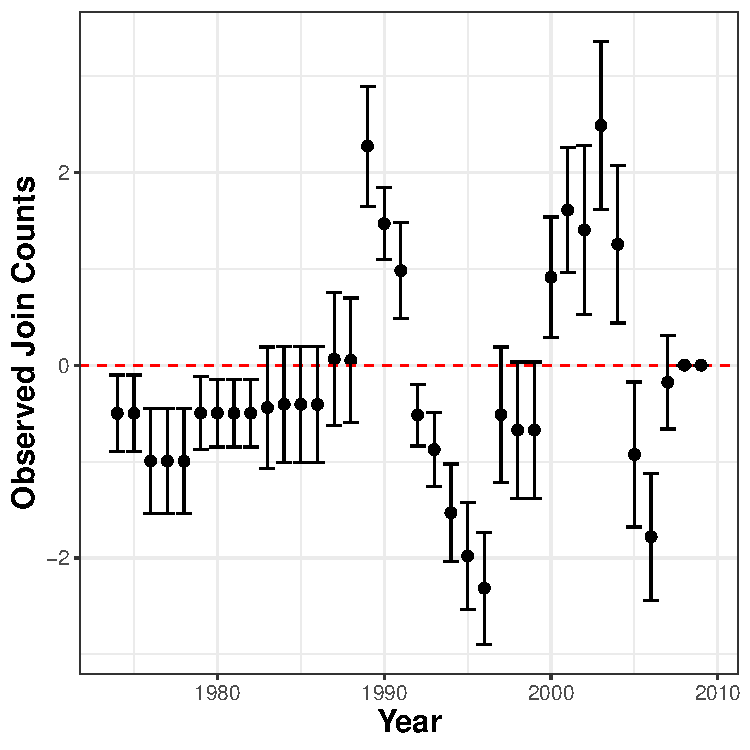
\includegraphics[width=\textwidth]{figures/JCnew.pdf}
         \caption{Join Count}
         \label{fig: joint count}
     \end{subfigure}
     \hfill
     \begin{subfigure}[b]{0.487\textwidth}
         \centering
         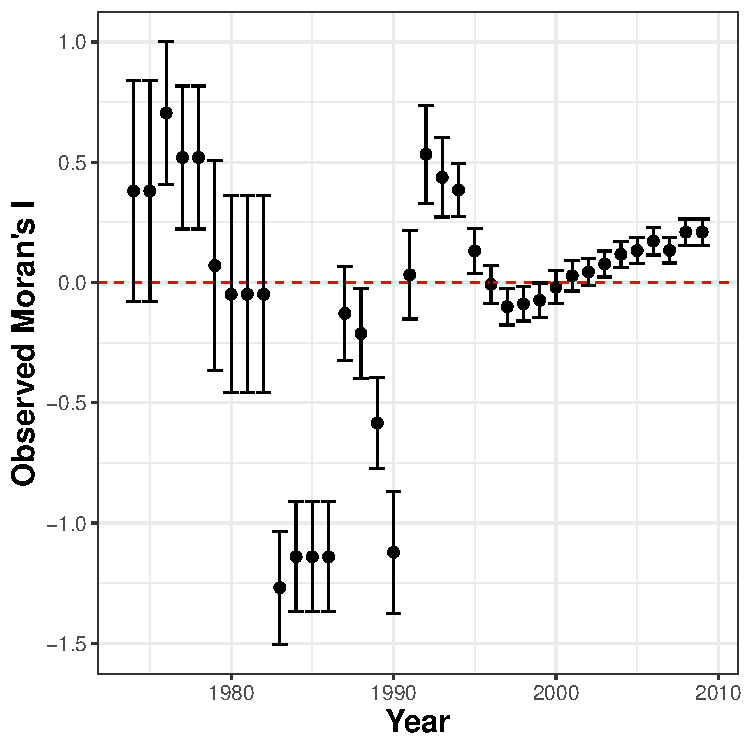
\includegraphics[width=\textwidth]{figures/MInew.pdf}
         \caption{Moran's I}
         \label{fig:moran's.I}
     \end{subfigure}
     \hfill
     \caption{Pre-estimation Spatial Autocorrelation Tests}
        \label{figure1: pre-estimation tests}
\end{figure}


\noindent Negative values indicate clustering (positive spatial autocorrelation), and positive values indicate spatial dispersion. Figure \ref{fig: joint count} clearly depicts spatially correlated patterns of potential “peace consolidation,” though the direction of the autocorrelation varies over time.

The second function, \code{plot\_Moran.I()}, implements the Global Moran’s I test, which assesses the direction and degree of spatial autocorrelation in continuous or ordinal data \citep{moran1950notes,ape}. We use this test to examine whether the duration of post-civil war peace among geographically proximate countries exhibits spatial autocorrelation (or dispersion). Like the previous function, \code{plot\_Moran.I()} plots the Moran’s I values based on user-defined adjacencies and, in this case, 90\% confidence intervals for each year. 

\begin{example}
plot_Moran.I(data = walter[[1]], var_duration = "duration", var_id = "ccode",
            var_time = "year", n = 12)
\end{example}

\noindent Figure \ref{fig:moran's.I} reveals that the spatial relationship of post-war peace survival oscillates between positive autocorrelation (in the 1970s, early 1990s, and late 2000s) and spatial dispersion (in much of the 1980s and late 1990s). Taken together, the Join Count and Moran’s I tests suggest that unobserved heterogeneous risk factors that transcend the borders of a single state may lead to spatial autocorrelation in both the consolidation and duration of post-war peace in \citeauthor{walter2015bad}'s (\citeyear{walter2015bad}) data. This suggests that a Spatial SP survival model is an appropriate method of analysis, particularly if proximate countries share common unobservable risk factors that affect their odds of being immune to war recurrence or the time it takes for renewed war to occur. 

\subsection {Applying the Bayesian Spatial SP survival model}

The \code{spatialSPsurv()} function fits the Bayesian Spatial SP survival model, which includes spatially autocorrelated frailties in the model’s split and survival stage and can incorporate time-varying covariates. We illustrate the features of the \code{spatialSPsurv()} function by fitting the Bayesian Spatial \emph{Weibull} cure model on \citeauthor{walter2015bad}'s (\citeyear{walter2015bad}) data on post-war peace.\footnote{The results for all models were calculated in \textbf{R} version 4.0.3. on a PC with a 6-core i7 processor.} The log-logistic results are reported in \citet{Bolte2021}. We include the \code{lgdpl} variable in the estimated model’s split-stage equation, which estimates the probability of units being in the “consolidated” post-war peace group (the “immune” fraction), though it is important to note that  \code{atrisk} is used here as the dependent variable. We estimate the probability of post-war survival among the at-risk fraction as a function of UN peacekeeping (\code{unpko}), outright military victory in the previous war (\code{victory}), the resolution of the previous war via peace agreement (\code{comprehensive}), and, again, GDP/capita (\code{lgdpl}). The spatial relationship of each country is incorporated into the model via the spatial weights matrix generated from the \code{spatial\_SA()} function described earlier.

The Spatial SP survival model is fit via Bayesian methods for inference. The MVN prior is used for the model’s split-stage ($\gamma$) and survival-stage ($\beta$) parameters (with the following hyperparameters $s_\beta = I_{p1}$, $v_\beta=p1$, $s_\gamma = I_{p2}$, $v_\gamma=p2$). The Gamma prior is used for the hazard’s shape parameter $\rho$ (with hyperparameters $a\rho=1$, $b\rho=1$), and separate CAR priors---with the Gamma hyperprior assigned to $\lambda$ for CAR ($\lambda$)\footnote{With vague prior $\left(a_{\lambda},b_{\lambda}\right)=\left(0.001,1/0.001\right)=\left(0.001,1000\right)$ as done for $\rho$}  ---incorporate the spatially autocorrelated frailties in the model’s split-stage (\code{V}) and survival stage (\code{W}). Estimation proceeds via the MCMC algorithm described in the previous section. To this end, we specify the MCMC sampler as follows: the argument \code{N = 15,000} sets the number of MCMC iterations to 15,000, \code{burn = 5,000} discards the first 5,000 states of the Markov chain, \code{thin = 15} specifies the number of steps that are employed to prevent autocorrelation, and \code{m = 10} limits the steps in the slice sampling to 10. The argument \code{w = c(1,1,1)} specifies the default values of the size of the slice sampling for $\gamma$, $\beta$, and $\rho$. 

For simplicity, we retain the default 0 as the initial value for all parameters with the \code{ini.beta}, \code{ini.gamma}, \code{ini.W}, and \code{ini.V} arguments. We incorporate separate proposal variances, namely \code{prop.varV = 1e-05} and \code{prop.varW = 1e-05}, for the split and survival stage frailties (\textbf{V}, \textbf{W}) and then assign separate Metropolis-Hastings proposal steps for estimating these parameters to optimize the acceptance rates. To specify the covariates in the model, \code{duration \textasciitilde} precedes the survival-stage covariates, while \code{immune \textasciitilde} precedes the split-stage variables. \code{Y0} indicates the time elapsed since inception until time t - 1, while \code{LY} is a dummy that captures the last observation year due to censoring or failure. \code{A = walter[[2]]} calls the spatial weights matrix from our list object.  \code{S= 'sp\_id'} (generated by \code{spatial\_SA())} gives the unit identifier in the spatial weights matrix that matches the units in the data frame. The argument \code{form} is used to specify the parametric survival distribution (which can be either ``Weibull'' or ``loglog'').  

Importantly, the model functions in the \pkg{BayesSPsurv} package generate single chains for each parameter, but we provide a routine for estimating multiple chains in parallel on the GitHub repository for the package (\url{https://github.com/Nicolas-Schmidt/BayesSPsurv}). We first discuss the results and diagnostics for the single-chain results using the above MCMC specification and then illustrate the multiple-chain results and diagnostics for the Spatial SP survival model. 

\begin{example}
set.seed(123456)
model <-  spatialSPsurv(duration = duration ~ victory + comprehensive + lgdpl + unpko ,
                            immune = atrisk ~ lgdpl,
                            Y0 = 't.0',
                            LY = 'lastyear',
                            S = 'sp_id' ,
                            data = walter[[1]],
                            N = 15000,
                            burn = 5000,
                            thin = 15,
                            w = c(1,1,1),
                            m = 10,
                            ini.beta =  0,
                            ini.gamma = 0,
                            ini.W = 0,
                            ini.V= 0,
                            form = "Weibull",
                            prop.varV = 1e-05,
                            prop.varW = 1e-05,
                            A = walter[[2]])
\end{example}

\noindent The function automatically provides a progress bar for users to track the percent of the computation that has been completed. The elapsed run time for the Spatial SP Weibull specification being examined here was just under 23 minutes (calculated with \code{system.time()}). Once completed, the generic \code{print()} function displays the results\footnote{95\% Bayesian Credible Intervals are reported in \citet{Bolte2021}.}: 

\begin{example}
print(model)

Call:
spatialSPsurv(duration = duration ~ victory + comprehensive + 
    lgdpl + unpko, immune = atrisk ~ lgdpl, Y0 = "t.0", 
    LY = "lastyear", S = "sp_id", A = walter[[2]], 
    data = walter[[1]], N = 15000, burn = 5000, thin = 15, w = c(1, 
        1, 1), m = 10, ini.beta = 0, ini.gamma = 0, ini.W = 0, 
    ini.V = 0, form = "Weibull", prop.varV = 1e-05, prop.varW = 1e-05)


Iterations = 1:666
Thinning interval = 1 
Number of chains = 1 
Sample size per chain = 666 

Empirical mean and standard deviation for each variable,
plus standard error of the mean:


Duration equation: 
                   Mean        SD    Naive SE Time-series SE
(Intercept)   0.3434823 1.0681878 0.041391437    0.078812901
victory       0.1028612 0.5321456 0.020620224    0.020620224
comprehensive 0.2036460 0.6178274 0.023940326    0.023940326
lgdpl         0.4831914 0.1424928 0.005521485    0.009230762
unpko         0.3057078 0.7695278 0.029818596    0.029818596

Immune equation: 
                  Mean       SD  Naive SE Time-series SE
(Intercept) -0.4306327 4.545655 0.1761405      0.3648687
lgdpl       -2.4722920 3.113144 0.1206319      0.1646276
\end{example}



\noindent The posterior mean estimates suggest that peace agreements, military victory, and peacekeeping units may increase the survival of post-civil war peace, though none of these parameters are highly reliable given their 95\% BCIs, as reported in \citep{Bolte2021}. However, \code{lgdpl} appears to reliably \textit{increase} the survival of peace among at-risk cases while also reliably \textit{decreasing} the probability of peace ``consolidation'' in the split-stage. Calling the \code{SPstats()} function calculates the Deviance Information Criterion (DIC) and log-likelihood (LL) statistics from the estimated model, where 
$DIC = -2 \times (L-P)$, $L$ is the log-likelihood of the data given the posterior means of the covariate parameters, and $P$ is the effective number of parameters in the model.

\begin{example}
SPstats(model)

$DIC
[1] -1726.128

$Loglik
[1] 5301.714

\end{example}

The \code{spatialSPsurv()} function produces an object of class \code{"mcmc"}, which is compatible with all standard summary and diagnostic methods for the single Markov chains in the \CRANpkg{coda} package \citep{coda-manual}. For instance, we can test for convergence with both the  \citet{geweke1992} test using the \code{geweke.diag()} function and the \citet{heidelberger1983} stationarity test via the \code{heidel.diag()} function in \CRANpkg{coda}. We report the \citet{heidelberger1983} stationarity test results in \citet{Bolte2021} to save space. In this case, the Geweke tests indicate little evidence against convergence for each split-stage and survival-stage covariate, because the test statistics are reasonably close to zero.

\begin{example}
geweke.diag(model$gammas)

Fraction in 1st window = 0.1
Fraction in 2nd window = 0.5 

(Intercept)       lgdpl 
    -1.3755      0.4429 

geweke.diag(model$betas)

Fraction in 1st window = 0.1
Fraction in 2nd window = 0.5 

  (Intercept)       victory comprehensive         lgdpl         unpko 
      -0.8248       -0.4271        1.8237        0.3601       -0.9471 

geweke.diag(model$rho)

Fraction in 1st window = 0.1
Fraction in 2nd window = 0.5 

  var1 
0.3544 

\end{example}

\noindent \CRANpkg{coda}'s \code{plot()} function can then be used to display trace and posterior density plots for the single Markov chains of the model's split-stage $\gamma$, survival-stage $\beta$, and $\rho$ parameters (which we do not report here to save space). Users may also wish to validate MCMC convergence using multiple chains with different initial values for each parameter rather than only examining single-chain diagnostics. A routine for generating multiple chains in parallel using the \CRANpkg{doParallel} \citep{doparallel} and \CRANpkg{doRNG} \citep{dorng} packages is available on the \pkg{BayesSPsurv} GitHub repository, though single chains with different starting values can also be run sequentially. The user can then collect them into a single \code{mcmc.list} object and easily plot the trace and density plots of the multiple chains. Using the code on GitHub, the Spatial SP survival model was re-run four times (to generate four chains) with 0, 1, 10, and 50 as the initial starting values for each of the estimated parameters ($\beta$, $\gamma$, $\textbf{W}$, and $\textbf{V}$). The trace and density plots for the multiple chains are reported below (we excluded the $\beta$ intercept for aesthetic reasons), and the total run time was approximately 28 minutes for all four chains to be generated simultaneously. 

\begin{example}
par(mfrow=c(2,2))
plot(gammas, density = FALSE, auto.layout = FALSE, col =c (28,26,27,29))
plot(gammas, trace = FALSE, auto.layout = FALSE)

par(mfrow=c(2,4))
plot(betas[,2:5], density= FALSE, auto.layout = FALSE, col = c(28,26,27,29))
plot(betas[,2:5], trace= FALSE, auto.layout = FALSE)
\end{example}


\begin{figure}[!htb]
\begin{center}
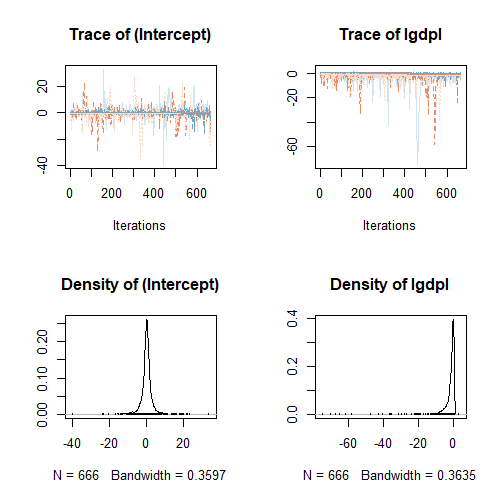
\includegraphics[width=0.65\textwidth]{figures/gammamultiple.png}

\end{center}
\caption{Posterior Densities of Bayesian Spatial Split-stage Parameters ($\gamma$)}
\label{figurey}
\end{figure}



\begin{figure}[!htb]
\begin{center} 
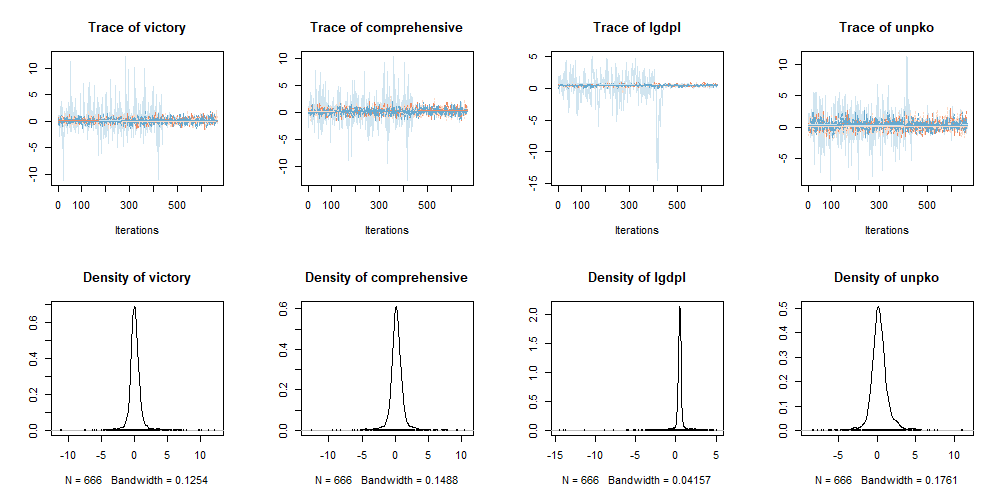
\includegraphics[width=\textwidth]{figures/betamultiple.png}
\end{center}
\caption{Posterior Densities of Bayesian Spatial Survival-stage Parameters ($\beta$)}
\label{figurex}
\end{figure}

The trace plots for the Spatial SP Weibull model's $\beta$ and $\gamma$ reveal decent mixing between the first three chains, though the fourth chain appears to take longer to converge. This is unsurprising given its extreme initial value. We can assess the convergence of the multiple chains using the Gelman-Rubin diagnostic, which compares the within-chain variance to the between-chain variance \citep{gelman}. If the difference in these variances is large, then the multiple chains likely have not converged to a proper stationary distribution. We can easily calculate the potential scale reduction factor (PSRF) with the \code{gelman.diag()} function in \pkg{coda}, which should be approximately 1 if all chains have converged to a common distribution. 

\begin{example}
Potential scale reduction factors:

              Point est. Upper C.I.
(Intercept)         1.19       1.38
victory             1.17       1.20
comprehensive       1.17       1.19
lgdpl               1.32       2.40
unpko               1.11       1.14

Multivariate psrf

1.05
\end{example}
 
\begin{example}
Potential scale reduction factors:

            Point est. Upper C.I.
(Intercept)       1.05       1.07
lgdpl             1.14       1.33

Multivariate psrf

1.05

\end{example}

\noindent The multivariate PSRF is less than 1.1 in both stages, but the point estimates for all parameters are still insufficiently far from 1, suggesting that extending the chains would likely improve the accuracy of the estimates.




One way to substantively interpret the spatial frailties is to display a map and determine whether adjacent units share similar frailty values (e.g., \citealp{darmofal2009bayesian}). The following code from the \CRANpkg{countrycode} \citep{countrycode-package} and \CRANpkg{rworldmap} \citep{rworldmap-package} packages permits users to create choropleth maps of the spatial frailty posterior means. Figures \ref{fig: V}-\ref{fig:W} display the single-chain split-stage (\code{V}) and survival-stage (\code{W}) frailties from our Spatial SP Weibull model (the code generates Figure \ref{fig: V}; Figure \ref{fig:W} simply uses \code{W} in place of \code{V}. 


\begin{example}
library(rworldmap)
library(countrycode)
library(classInt)

spv  <- matrix(apply(model$V, 2, mean), ncol = 1, nrow = ncol(model$V))
ISO3 <- countrycode(colnames(model$V) ,'gwn','iso3c')
spv  <- data.frame(ccode = colnames(model$V), ISO3 = ISO3, spv = spv)
map  <- joinCountryData2Map(spv, joinCode = "ISO3", nameJoinColumn = "ISO3")
classInt <- classIntervals(map[["spv"]], n = 6, style = "quantile")
mapParams <- mapCountryData(map,
                            nameColumnToPlot = "spv",
                            addLegend = FALSE,
                            catMethod = classInt[["brks"]],
                            colourPalette = palette(RColorBrewer::brewer.pal(6,"RdBu")),
                            mapTitle = "")

do.call(addMapLegend, c(mapParams, legendLabels = "all", legendWidth = 0.5,
                                   legendIntervals = "data", legendMar = 2))
\end{example}

%Figure 5
\begin{figure}[!htb]
     \centering
     \begin{subfigure}[b]{0.495\textwidth}
         \centering
         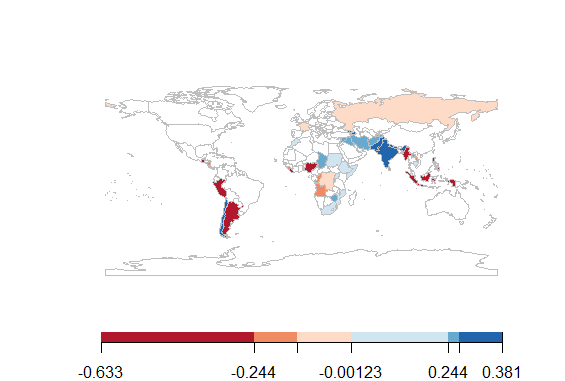
\includegraphics[width=\textwidth]{figures/spatial_VmapNEW.png}
         \caption{Split-stage (\textbf{V})}
         \label{fig: V}
     \end{subfigure}
     \hfill
     \begin{subfigure}[b]{0.495\textwidth}
         \centering
         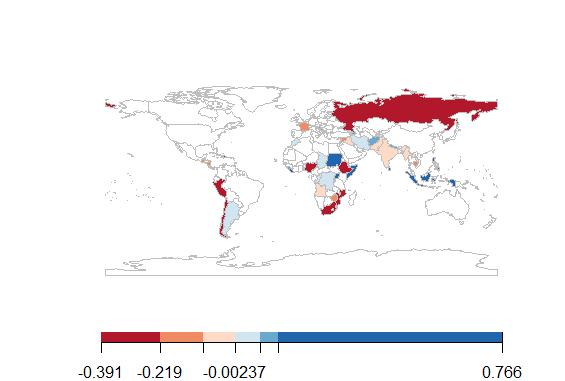
\includegraphics[width=\textwidth]{figures/spatial_WmapNEW.png}
         \caption{Survival-stage (\textbf{W})}
         \label{fig:W}
     \end{subfigure}
     \hfill
     \caption{Spatial Frailty Posterior Means}
        \label{figure5:choropleth maps}
\end{figure}

\noindent Note that in certain regions, there are distinct spatial bands in the (i) split-stage frailties, which range from -0.633 to 0.381 with a corresponding standard deviation of 0.34 and (ii) survival-stage frailties that range from -0.391 to 0.766 with a corresponding standard deviation of 0.32. These spatial bands reveal geographic clustering in both consolidation and duration of post-war peace since similar frailty values often occur near one another.

\subsection{Applying the Bayesian Exchangeable and Pooled SP survival models}

The \pkg{BayesSPsurv} package can also be used to estimate Bayesian Exchangeable and Pooled SP survival models. The Exchangeable model incorporates frailties that are assumed to be statistically independent in both stages, while the Pooled model excludes frailties altogether. We again use \citeauthor{walter2015bad}'s (\citeyear{walter2015bad}) data on post-civil war peace to illustrate these models. Beginning with the Exchangeable Weibull SP survival model, we again assign the MVN prior to the model’s $\gamma$ and $\beta$ parameters, the Gamma prior to $\rho$, and the same default settings for the hyperparameters ($s_\beta = I_{p1}$, $v_\beta=p1$, $s_\gamma = I_{p2}$, $v_\gamma=p2$,   $a_\rho = 1$, $b_\rho = 1$). We also incorporate separate proposal variance variables for the nonspatial i.i.d frailties ($V_i$,$W_i$) and assign separate Metropolis-Hastings steps to estimate these parameters. Further, we use almost the same MCMC sampler specification as before. However, rather than incorporating spatial information via an adjacency matrix, we let \code{id\_WV=country} to define the country-level nonspatial frailties.

\begin{example}
set.seed(123456)
country  <- countrycode(unique(walter[[1]]$ccode),'gwn','iso3c')
model1 <- exchangeSPsurv(duration = duration ~ victory + comprehensive + lgdpl + unpko,
                         immune = atrisk ~ lgdpl,
                         Y0 = 't.0',
                         LY = 'lastyear',
                         S = 'sp_id' ,
                         data = walter[[1]],
                         N = 15000,
                         burn = 5000,
                         thin = 15,
                         w = c(1,1,1),
                         m = 10,
                         ini.beta =  0,
                         ini.gamma = 0,
                         ini.W = 0,
                         ini.V= 0,
                         form = "Weibull",
                         prop.varV = 1e-05,
                         prop.varW = 1e-05,
                         id_WV=country)
\end{example}

\noindent Again, users can assess either single or multiple (parallel) Markov chains with different starting parameter values when fitting the Exchangeable SP survival model. We report the single-chain results here for simplicity. The run time for the above specification was approximately 16 minutes and 30 seconds. The single-chain results and model fit statistics are obtained with the \code{print()} and \code{SPstats()} functions.

\begin{example}
print(model1)

Call:
exchangeSPsurv(duration = duration ~ victory + comprehensive + 
    lgdpl + unpko, immune = atrisk ~ lgdpl, Y0 = "t.0", 
    LY = "lastyear", S = "sp_id", data = walter[[1]], 
    N = 15000, burn = 5000, thin = 15, w = c(1, 1, 1), m = 10, 
    ini.beta = 0, ini.gamma = 0, ini.W = 0, ini.V = 0, form = "Weibull", 
    prop.varV = 1e-05, prop.varW = 1e-05, id_WV = country)


Iterations = 1:666
Thinning interval = 1 
Number of chains = 1 
Sample size per chain = 666 

Empirical mean and standard deviation for each variable,
plus standard error of the mean:


Duration equation: 
                    Mean        SD    Naive SE Time-series SE
(Intercept)   0.31054460 1.0938158 0.042384501     0.08335381
victory       0.14520456 0.5328378 0.020647044     0.02064704
comprehensive 0.09721372 0.6374526 0.024700786     0.02470079
lgdpl         0.48473536 0.1455731 0.005640844     0.01061988
unpko         0.44731384 0.7421925 0.028759376     0.02875938

Immune equation: 
                  Mean       SD  Naive SE Time-series SE
(Intercept) -0.8993176 5.924550 0.2295716      0.4969172
lgdpl       -3.7286951 5.846367 0.2265421      0.5271203

SPstats(model1)
$DIC
[1] 3549.075

$Loglik
[1] 7506.608
\end{example}

\noindent Based on these results, \code{lgdpl} is still a highly reliable predictor of longer peace duration among conflicts at risk of recurrence, while the other survival stage covariates remain positive but statistically unreliable. In contrast to the spatial frailty model, however, the effect of \code{lgdpl} on the probability of peace consolidation is now statistically unreliable.  Users interested in displaying and interpreting the exchangeable frailties can do so in a variety of ways, but if these results are being compared to those of a spatial frailty model, we recommend mapping the exchangeable frailty values and comparing the clustering (or lack thereof) of the i.i.d. frailty terms to those produced from the spatial model \citep{darmofal2009bayesian}.

Finally, the \code{pooledSPsurv()} function fits the Pooled Bayesian SP survival model. For this application, we again assign the MVN prior to the model’s $\gamma$ and $\beta$ parameters, the Gamma prior to $\rho$, and the same default settings for the hyperparameters described earlier. 

\begin{example}
set.seed(123456)
model2 <- pooledSPsurv(duration = duration ~ victory + comprehensive + lgdpl + unpko,
                       immune = atrisk ~ lgdpl,
                       Y0 = 't.0',
                       LY = 'lastyear',
                       data = walter[[1]],
                       N = 15000,
                       burn = 5000,
                       thin = 15,
                       w = c(1,1,1),
                       m = 10,
                       ini.beta =  0,
                       ini.gamma = 0,
                       form = "Weibull")
\end{example}

\noindent Note that the MCMC sampler is almost identical to that of the previous two models, but we now \textit{exclude} the separate Metropolis-Hastings proposal step for the frailities in the MCMC algorithm as well as the initial values for the frailty estimates since this is a non-frailty model. The run time for the Pooled model was approximately 10 minutes. The single-chain output is again easily displayed.

\begin{example}
print(model2)

Call:
pooledSPsurv(duration = duration ~ victory + comprehensive + 
    lgdpl + unpko, immune = atrisk ~ lgdpl, Y0 = "t.0", 
    LY = "lastyear", data = walter[[1]], N = 15000, burn = 5000, 
    thin = 15, w = c(1, 1, 1), m = 10, ini.beta = 0, ini.gamma = 0, 
    form = "Weibull")


Iterations = 1:666
Thinning interval = 1 
Number of chains = 1 
Sample size per chain = 666 

Empirical mean and standard deviation for each variable,
plus standard error of the mean:


Duration equation: 
                   Mean        SD    Naive SE Time-series SE
(Intercept)   0.3014335 1.0572594 0.040967971     0.07197438
victory       0.1060453 0.5485730 0.021256770     0.02125677
comprehensive 0.1900127 0.6054421 0.023460406     0.02481878
lgdpl         0.4647260 0.1552465 0.006015679     0.01166616
unpko         0.2692275 0.7740804 0.029995006     0.02999501

Immune equation: 
                 Mean       SD  Naive SE Time-series SE
(Intercept) -1.213902 9.617551 0.3726725      1.3195278
lgdpl       -2.896038 4.939374 0.1913968      0.5267751


SPstats(model2)

$DIC
[1] 1804.527

$Loglik
[1] 6229.248
\end{example}

For both the Exchangeable and Pooled SP survival models, users can again employ the code and routines available in our GitHub repository to view the trace plots from the single or multiple Markov chains associated with the posterior densities for the $\gamma$, $\beta$, and $\rho$ parameters and conduct any relevant convergence diagnostics. The plots and convergence test statistics for the models presented here are reported in \citet{Bolte2021} to save space. Additional information is available at \url{https://github.com/Nicolas-Schmidt/BayesSPsurv}. 

\section{Conclusion}
Survival data often include two populations with different underlying risk propensities: the immune fraction of right-censored units that will never experience the event of interest and the at-risk fraction of units that have or will. Numerous R-packages such as \CRANpkg{smcure}, \CRANpkg{nltm}, and \CRANpkg{spduration} have been developed to fit parametric or semi-parametric cure models for nonspatial survival data, but none of these packages allow the user to account for spatial autocorrelation in both stages. A separate set of packages allows the user to include spatially weighted frailties in conventional survival models \citep{taylor2017spatsurv, spBayesSurv-article}, but spatial autocorrelation may also influence the probability of immunity from an event of interest. The \pkg{BayesSPsurv} package addresses this lacuna by offering a suite of functions to fit Bayesian SP survival models. Specifically, users can estimate Bayesian Pooled, Exchangeable, and Spatial frailty SP survival models with time-varying covariates, specify their own spatial weights matrices, and easily examine diagnostic statistics. The applied potential of the Spatial SP survival model, in particular, is considerable, as researchers studying anything from the survival of cancer patients to the survival of political regimes may have a methodological need to model spatial autocorrelation in the immune fraction. 

Future work can build upon the spatial and nonspatial cure models presented here to develop estimation routines for survival data with multiple stages, competing risks, or recurrent events. Moreover, although \pkg{BayesSPsurv}  is the first to allow spatially autocorrelated frailties in both stages, future work can extend the frailty models in our package by employing a similar approach as \citet{yin} to incorporate shared frailties with factor loadings to account for any correlation between the frailty terms ($\textbf{W}$ and $\textbf{V}$) in either stage. Subsequent iterations of the package will include alternative baseline hazards based on penalized splines or nonparametric Gaussian processes as well as the option to use a semiparametric Cox model with exchangeable or spatial frailties. Implementing these future developments with an external MCMC sampling dependency built on C++ subroutines like STAN would be useful, given the Hamiltonian Monte Carlo algorithm's efficiency in sampling from high dimensional posterior distributions. We also plan to extend \pkg{BayesSPsurv} to accommodate left and interval censoring and delayed entry. 

\bibliography{bolte-etal-spatSP.bib}

\address{Brandon Bolte\\
Department of Political Science\\
Penn State University\\
USA\\
\email{blb72@psu.edu}}

\address{Nicol\'as Schmidt\\
Department of Political Science\\
Universidad de la Rep\'ublica\\
Uruguay\\
\email{nschmidt@cienciassociales.edu.uy}}

\address{Sergio B\'ejar\\
Department of Political Science\\
San Jos\'e State University\\
USA\\
\email{sergio.bejar@sjsu.edu}}

\address{Nguyen Huynh\\
Department of Political Science\\
Penn State University\\
USA\\
\email{nkh8@psu.edu}}

\address{Bumba Mukherjee\\
Department of Political Science\\
Penn State University\\
USA\\
\email{sxm73@psu.edu}}


